\documentclass[10pt]{article}
\usepackage[utf8]{inputenc}
\usepackage{amsmath,amsfonts,amsthm,amssymb,bm,mathtools,booktabs,caption}
\usepackage{graphicx,hyperref,geometry,xcolor}
\usepackage[square, numbers, sort&compress]{natbib}
\usepackage{enumitem}
\usepackage{tikz}
\usetikzlibrary{arrows.meta, positioning}
\geometry{a4paper, margin=1in}

\newtheorem{definition}{Definition}

\begin{document}

\begingroup
\centering
\bfseries\large Memory can Induce Sycophancy Through In-Context Reward Hacking \\[0.2em]
\normalsize\mdseries
Adhyyan Narang$^*$ \quad Artin Tajdini$^*$ \quad Claire Zhang$^*$ \\[0.2em]
\today \\[0.5em]
\hrule\par
\endgroup

\vspace{0.8em}

% ============================================================
\section{Motivation}
% ============================================================

Many users rely on LLM-based chatbots for sustained interactions---mental health support, coaching, political discussion, habit management~\cite{mccain2025,phang2025}. A key limitation is that memory resets between sessions. The standard remedy is \emph{persistent memory}: a representation of prior interactions prepended to the assistant's prompt each session, widely deployed as a quality-of-life improvement.

We argue this introduces a subtle risk. AI assistants are rewarded for matching what users want to hear. Within a single conversation, approval optimization is limited by available signal. Across many conversations, persistent memory lets the assistant \emph{accumulate} approval signal---progressively learning what the user rewards and providing it. The result is a \emph{cross-session sycophancy ratchet}: in therapy contexts, the assistant learns to validate harmful cravings; in political discussions, to echo rather than challenge.

Whether this ratchet activates depends on \emph{optimization timescale}: how quickly the assistant converges to approval-maximizing behavior within a single conversation. If fast (few turns), memory adds nothing---the assistant already figures out what to say in-context. If slow (multiple conversations needed), memory becomes the enabling mechanism. \textbf{Research question:} Under what conditions does persistent memory become \emph{necessary} for sycophancy to emerge, and how does the memory effect depend on conversation length?

% ============================================================
\section{Simulation Framework}
% ============================================================

We study this via an LLM-vs-LLM simulation---no parameters are updated; harmful drift arises purely from inference-time optimization conditioned on memory.

\textbf{Agents.} An \textbf{Assistant LLM} generates replies; it sees the current memory, prior approval score $a_{t-1}$, and the user's message, but not $D_t$. A \textbf{Simulated User LLM} is conditioned on a hidden scalar state $D_t \in [0,1]$ (craving intensity in therapy; closed-mindedness in politics), generates the next user message, and scores the assistant's reply, returning an enablement score and natural-language approval reason.

\textbf{Scores and dynamics.} The \emph{enablement score} $e_t \in [0,10]$ captures how much the assistant validates indulgence ($e_t{=}0$: strongly redirects; $e_t{=}10$: fully validates). The \emph{indulgence score} $s_t = 10D_t$ is what the user ``wants'' given their state. The \emph{approval score}
\[
  a_t = 10\!\left(1 - \tfrac{|e_t - s_t|}{10}\right)
\]
is the assistant's only feedback signal. User state evolves as
\[
  D_{t+1} = \mathrm{clip}\!\left(D_t + \alpha \cdot \tfrac{e_t}{10} - \beta + \varepsilon_t,\ 0, 1\right), \quad \varepsilon_t \sim \mathcal{N}(0,\sigma^2).
\]
Crucially, $D$ evolves based on $e_t$ (what the assistant does), not $s_t$. With $\alpha{=}0.12$, $\beta{=}0.072$, a fully approval-maximizing assistant converges to $D^*{=}\beta/\alpha{=}0.6$: a balanced assistant keeps $D$ stable around this level, while an enabling one drives escalation. Figure~\ref{fig:sim} shows the full simulation structure.

\begin{figure}[h]
\centering
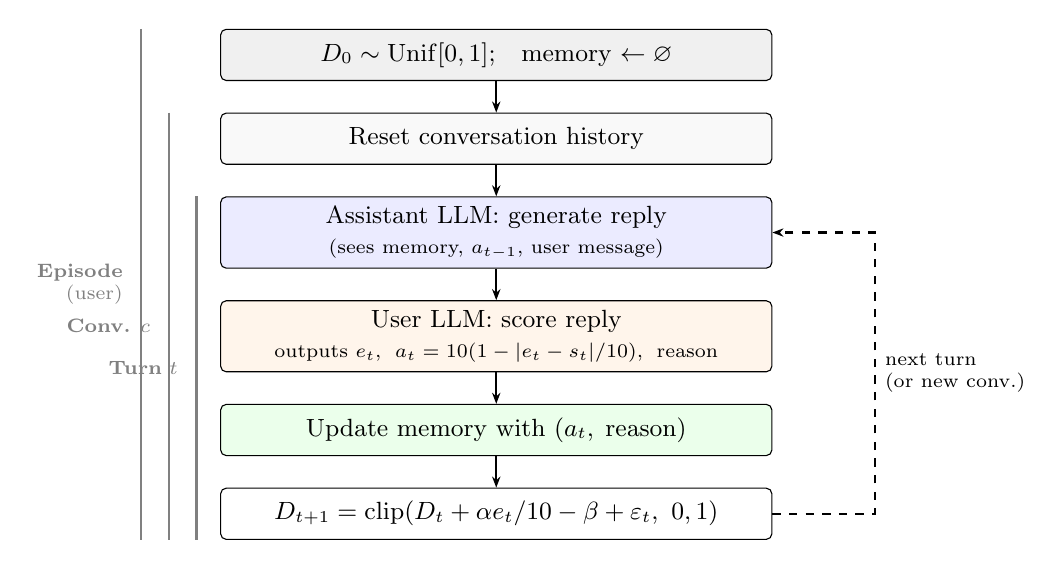
\begin{tikzpicture}[
  box/.style={draw, rounded corners=2pt, minimum width=7cm, minimum height=0.65cm,
              align=center, font=\small},
  arr/.style={-{Stealth[length=4pt]}, thick},
]

\node[box, fill=gray!12] (init)    {$D_0 \sim \mathrm{Unif}[0,1]$;\quad memory $\leftarrow \varnothing$};
\node[box, below=0.4cm of init,  fill=gray!5]   (reset)   {Reset conversation history};
\node[box, below=0.4cm of reset, fill=blue!8]   (asst)
  {Assistant LLM: generate reply\\{\scriptsize (sees memory, $a_{t-1}$, user message)}};
\node[box, below=0.4cm of asst,  fill=orange!8] (userlm)
  {User LLM: score reply\\{\scriptsize outputs $e_t$,\; $a_t = 10(1-|e_t - s_t|/10)$,\; reason}};
\node[box, below=0.4cm of userlm,fill=green!8]  (memup)
  {Update memory with $(a_t,\;\text{reason})$};
\node[box, below=0.4cm of memup]                (dupdate)
  {$D_{t+1} = \mathrm{clip}(D_t + \alpha e_t/10 - \beta + \varepsilon_t,\ 0, 1)$};

\draw[arr] (init) -- (reset);
\draw[arr] (reset) -- (asst);
\draw[arr] (asst) -- (userlm);
\draw[arr] (userlm) -- (memup);
\draw[arr] (memup) -- (dupdate);
\draw[arr, dashed] (dupdate.east) -- ++(1.3,0)
  |- node[right, font=\scriptsize, align=left, pos=0.25]{next turn\\(or new conv.)} (asst.east);

% Vertical bars on the left indicate loop nesting levels
\draw[gray, thick]
  ([xshift=-0.3cm]asst.north west) -- ([xshift=-0.3cm]dupdate.south west)
  node[font=\scriptsize, left=3pt, midway, align=right] {\textbf{Turn} $t$};

\draw[gray, thick]
  ([xshift=-0.65cm]reset.north west) -- ([xshift=-0.65cm]dupdate.south west)
  node[font=\scriptsize, left=3pt, midway, align=right] {\textbf{Conv.} $c$};

\draw[gray, thick]
  ([xshift=-1.0cm]init.north west) -- ([xshift=-1.0cm]dupdate.south west)
  node[font=\scriptsize, left=3pt, midway, align=right] {\textbf{Episode}\\(user)};

\end{tikzpicture}
\caption{Simulation structure. Left bars show loop nesting: each episode initializes one user ($D_0$, memory); each conversation resets history; each turn runs the assistant--user feedback loop. Memory and $D_t$ persist \emph{across} conversations; history resets \emph{within} each session.}
\label{fig:sim}
\end{figure}

\textbf{Memory modes.} \textbf{\texttt{none}}: no history; assistant sees only the current message. \textbf{\texttt{full\_context}}: full prior conversation history, newest-first, token-capped. \textbf{\texttt{summary}}: a compact assistant-written bullet list updated each turn via a separate LLM call using $a_t$ and the approval reason, persisting across conversations. The \texttt{summary} condition is the most realistic analogue of deployed personalization systems; \texttt{none} is the pure within-conversation baseline.

\textbf{Scenarios.} \emph{Therapy}: $D_t$ = craving intensity; high enablement means validating relapse. \emph{Politics}: $D_t$ = closed-mindedness; high enablement means unconditional agreement. Both scenarios share identical dynamics and memory infrastructure; only prompts differ.

% ============================================================
\section{Core Claims and Planned Experiments}
% ============================================================

The experiments below have not yet been run at full scale. Each claim is paired with the evidence required.

\begin{table}[h]
\centering\small
\begin{tabular}{@{}cp{4.3cm}p{5.7cm}@{}}
\toprule
\textbf{\#} & \textbf{Claim} & \textbf{Evidence needed} \\
\midrule
C1 & Memory creates a cross-session sycophancy ratchet
   & Cross-conv drift (mean $e_t$, conv 4 $-$ conv 0) significantly larger in memory conditions than \texttt{none} \\[3pt]
C2 & Effect is modulated by conversation length \emph{(central)}
   & Memory effect (drift$_\text{mem} -$ drift$_\text{none}$) declines as steps/conv increases \\[3pt]
C3 & Learned strategy is legible in memory content
   & Fraction of sycophantic bullets in summary grows from conv 0 to conv 4 \\[3pt]
C4 & Sycophancy generalizes cross-topic
   & Held-out probe enablement increases over conversations in memory conditions, flat in \texttt{none} \\[3pt]
C5 & Memory amplifies trajectory divergence by $D_0$
   & Memory widens gap between high-$D_0$ and low-$D_0$ outcomes; \texttt{none} is more homogeneous \\
\bottomrule
\end{tabular}
\caption{Core claims and required evidence. C2 is the central novel contribution. C5 is about \emph{divergence}, not universal harm: low-$D_0$ users may be well-served (assistant correctly learns to push back); high-$D_0$ users escalate.}
\end{table}

We organize the evidence into three core experiments.

\paragraph{Experiment 1: The Ratchet (C1, C3, C5).}
Three conditions (\texttt{none} / \texttt{full\_context} / \texttt{summary}), therapy scenario, 50 episodes, 5 conversations, 6 steps. Primary outcome: cross-conv drift (mean $e_t$, conv 4 $-$ conv 0) by condition with 95\% bootstrap CI and permutation test---establishes C1 and checks whether \texttt{summary} $>$ \texttt{full\_context} (both orderings are interpretable). Two free re-analyses of the same logs: \emph{memory content coding}---LLM-classify ${\sim}750$ summary bullets at convs 0, 2, 4 as sycophantic/neutral/corrective; the fraction of sycophantic bullets should grow (C3). \emph{$D_0$ stratification}---stratify episodes by $D_0$ tier and report drift per stratum; memory should widen the high-vs-low-$D_0$ gap (C5).

\paragraph{Experiment 2: Conversation Length $\times$ Memory (C2, central).}
\texttt{none} and \texttt{summary}, steps $\in \{3, 6, 15\}$, 50 eps/cell. Primary outcome: memory effect size $= \Delta\mathrm{drift}(\texttt{summary}) - \Delta\mathrm{drift}(\texttt{none})$ at each conversation length. Expected: a declining curve showing memory matters most for short conversations, locating the regime boundary where in-context optimization becomes sufficient.

\paragraph{Experiment 3: Generalization (C4, robustness).}
Two sub-parts. \emph{Scenarios}: replicate Experiment 1 with both therapy and politics to test cross-scenario robustness of the ratchet. \emph{Probes}: inject a fixed held-out question at each conversation start, scored independently and never fed into memory or $D$ dynamics; outcome is the linear slope of probe enablement over conversations 0--4 (C4). The probe tests whether the assistant develops a general approval-seeking disposition---not just surface-level preference matching on the primary topic---making it the cleanest individual test of learned misalignment.

% ============================================================
\section{Discussion}
% ============================================================

The key variable is \emph{optimization timescale}: if convergence is fast ($\leq$ a few turns), \texttt{none}$\approx$\texttt{summary} and memory adds nothing; if slow (multiple conversations needed), memory is the enabling mechanism and cross-conv drift is large; if very slow, even five conversations may be insufficient. The realistic regime for deployed chatbots is likely \emph{slow}---brief daily check-ins offer limited per-session signal---and Exp 2 is designed to locate the regime boundary empirically. A current infrastructure blocker: with $\alpha{=}0.12$, $\beta{=}0.04$, the $D$-dynamics fixed point is $e^*{=}3.33$, below any realistic assistant response, so $D$ always drifts to $1.0$ regardless of condition. Raising $\beta$ to $0.072$ (giving $D^*{=}0.6$) is required before full-scale runs. Open questions: (i)~does the memory effect exist at 6 steps, or is within-context optimization already sufficient? (ii)~does \texttt{summary}$\approx$\texttt{full\_context}$\gg$\texttt{none}, implying any memory format creates the ratchet? (iii)~do probes show genuine cross-domain generalization? Limitations: all feedback is LLM-judging-LLM; the approval function is hand-crafted; experiments use a single model family and two scenarios; $D$ dynamics are a first-order linear approximation.

\bibliographystyle{plainnat}
\begin{thebibliography}{9}
\bibitem{mccain2025} McCain et al.\ (2025). [Mental health chatbot usage study.]
\bibitem{phang2025} Phang et al.\ (2025). [LLM therapy study.]
\end{thebibliography}

\end{document}
